% \newpage

\section{Experiments}

\textbf{Datasets.} We evaluate the performance of the LAC model on two datasets using a variety of evaluation metrics. The Pouring dataset \cite{2017_tcn}, which focuses on the action of pouring liquids, includes 70 training and 14 testing videos. The PennAction dataset \cite{2013_pennaction}, featuring 13 human actions, contains 1140 training and 966 testing videos. We utilize the key events and phases for the videos in both datasets as proposed by TCC \cite{2019_tcc}.


\noindent \textbf{Implementation Details.} 
Our encoder, \(f: \mathbb{R}^{TxCxWxH} \to Z\), maps video inputs $V$ into an embedding space \(Z\). We use a ResNet50-v2 \cite{2015_resnet} as our backbone to extract features from the Conv4c layer with an output size of \(10x10x512\).
These features are then processed through adaptive max pooling, followed by two fully connected layers with ReLU activation.
A subsequent linear layer projects the features into a 256-dimensional space. 
To enhance the model’s capacity to capture long-range dependencies, we integrate sine-cosine positional encoding and employ a two-layer Transformer encoder. 
 To improve the model’s ability to capture long-range dependencies, we incorporate sine-cosine positional encoding and apply a two-layer Transformer encoder. 
 The final embedding layer reduces the dimensionality to 128 for the frame-wise representations.

\begin{table}[]
\small
\centering
\begin{tabularx}{\textwidth}{X|ccc|ccc|c|c}
\multirow{2}{*}{\textbf{Method}} & \multicolumn{3}{c|}{\textbf{Class}} & \multicolumn{3}{c|}{\textbf{AP@K}} & \multirow{2}{*}{\textbf{Progress}} & \multirow{2}{*}{\textbf{$\tau$}} \\ 
\cline{2-7}
 & \textbf{10} & \textbf{50} & \textbf{100} & \textbf{K=5} & \textbf{K=10} & \textbf{K=15} & & \\ 
\hline
\hline
TCN \cite{2017_tcn}        & 80.32 & 81.44 & 83.56 & 76.26 & 76.71 & 77.26 &  82.30 & 83.51 \\
TCC \cite{2019_tcc}        & 86.60 & 86.78 & 86.86 & 81.84 & 80.94 & 81.69 &  83.36 & 85.26 \\
LAV \cite{2021_lav}        & 89.77 & 90.35 & 91.77 & 87.48 & 88.36 & 88.40 &  85.20 & 88.75 \\
GTA \cite{2021_gta}        & 89.34 & 90.20 & 90.22 & 87.79 & 87.48 & 87.82 &  88.67 & 92.47 \\
SCL \cite{2022_carl}       & \underline{92.76} & 92.80 & 93.05 & 88.75 & 88.51 & 88.97 & 91.26 & \underline{98.20} \\
LRPROP \cite{2024_lrprop}  & 92.70 & \underline{94.44} & \underline{94.36} & \underline{92.41} & \underline{90.33} & \underline{90.86} & \underline{94.09} & \textbf{99.46} \\
\hline
LAC & \textbf{95.87} & \textbf{95.78} & \textbf{95.16} & \textbf{92.76} & \textbf{91.07} & \textbf{91.37} & \textbf{94.24} & 97.50 \\
\hline
\hline
\end{tabularx}
\caption{Performance comparison of state-of-the-art methods on the Pouring Dataset \cite{2017_tcn}}
% \caption{Performance comparison of LAC and SOTA on the Pouring Dataset \cite{2017_tcn}}
\label{tab: p_class}
\end{table}



\noindent \textbf{Evaluation Metrics.}
% Following related work \cite{2019_tcc, 2021_lav, 2021_gta, 2022_carl, 2024_lrprop}, we freeze the model's weights and evaluate it using the following metrics: 
Following related work \cite{2019_tcc, 2021_lav, 2021_gta, 2022_carl, 2024_lrprop}, we evaluate our model using the following metrics:
(i) \textit{Phase Classification}, which assesses the accuracy of action phase predictions by training an SVM classifier on our embeddings;
(ii) \textit{Phase Progression}, which evaluates how accurately our embeddings predict action progress using a linear regression model's average R-squared value, based on normalized timestamp differences;
(iii) \textit{Average Precision@K (AP@K)}, which evaluates fine-grained frame retrieval accuracy by calculating the proportion of correctly matched phase labels within the K closest frames;
(iv) \textit{Kendall's Tau}, which quantifies the temporal alignment between sequences by comparing the ratio of concordant to discordant frame pairs.

\subsection{Results}

We apply the same four metrics to the Pouring dataset \cite{2017_tcn}. For the PennAction dataset \cite{2013_pennaction}, we evaluate each metric across all action categories and report the average results. 
To ensure a fair comparison, we replicated the evaluations of previous approaches using the GitHub repositories \footnote{github.com/google-research/google-research/tcc, github.com/trquhuytin/LAV-CVPR21,\\github.com/hadjisma/VideoAlignment, github.com/minghchen/CARL\_code} provided by the original authors. 
Each model was trained using its respective pre-trained backbone. 
An exception was made for LRPROP, as their GitHub repository is not available.

\noindent \textbf{Results on Pouring Dataset.} 
Table~\ref{tab: p_class} presents a comparison of our method's performance against state-of-the-art approaches on the Pouring dataset. Bold and underlined text denote the best and second-best results.
% Our method significantly outperforms prior work when using our embeddings for action recognition tasks (Table~\ref{tab: p_class}).
Notably, it achieves a +3.11\% improvement on Phase Classification using only 10\% of the labels. Additionally, our model excels in AP@K and Progress metrics.
However, we observe lower performance in Kendall's Tau. We hypothesize this is due to how the SW's algorithm encourages skipping unnecessary segments of the sequence. The introduction of gap open and extend penalties could disrupt the continuity needed for high Kendall's Tau scores.

\begin{table}[]
\small
\centering
\begin{tabularx}{\textwidth}{X|ccc|ccc|c|c}
\multirow{2}{*}{\textbf{Method}} & \multicolumn{3}{c|}{\textbf{Class}} & \multicolumn{3}{c|}{\textbf{AP@K}} & \multirow{2}{*}{\textbf{Progress}} & \multirow{2}{*}{\textbf{$\tau$}} \\ 
\cline{2-7}
 & \textbf{10} & \textbf{50} & \textbf{100} & \textbf{K=5} & \textbf{K=10} & \textbf{K=15} & & \\ 
\hline
\hline
TCN \cite{2017_tcn}        & 69.73 & 70.26 & 70.01 & 60.92 & 61.57 & 61.52 &  76.37 & 63.72 \\
TCC \cite{2019_tcc}        & 86.60 & 86.78 & 86.86 & 81.84 & 80.94 & 81.69 &  83.36 & 85.26 \\
LAV \cite{2021_lav}        & 88.51 & 88.72 & 88.97 & 73.47 & 73.13 & 74.27 &  92.52 & 93.06 \\
GTA \cite{2021_gta}        & 84.21 & 84.68 & 85.28 & 71.72 & 72.17 & 71.52 &  90.51 & 83.35 \\
SCL \cite{2022_carl}       & 87.85 & 87.52 & 88.15 & 91.70 & 90.61 & 90.58 &  92.89 & \underline{98.14}\\
LRPROP \cite{2024_lrprop}  & \underline{91.90} & \underline{92.96} & \underline{93.25} & \underline{92.46} & \underline{92.2} & \underline{92.03} & \underline{93.03} & \textbf{99.09} \\
\hline
LAC & \textbf{95.57} & \textbf{93.79} & \textbf{93.40} & \textbf{93.87} & \textbf{93.41} & \textbf{92.65} & \textbf{94.21} & 94.10 \\
\hline
\hline
\end{tabularx}
\caption{Performance comparison of state-of-the-art methods on the PennAction Dataset \cite{2013_pennaction}}
% \caption{Performance comparison of LAC and SOTA on the PennAction Dataset \cite{2013_pennaction}}
\label{tab: pn_class}
\end{table}

\begin{figure}[t]
\begin{tabular}{cc}
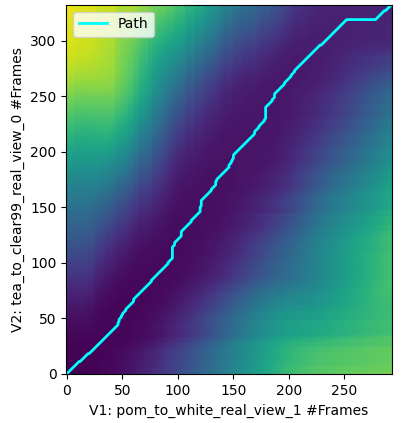
\includegraphics[width=0.195\textwidth]{images/v1.png}&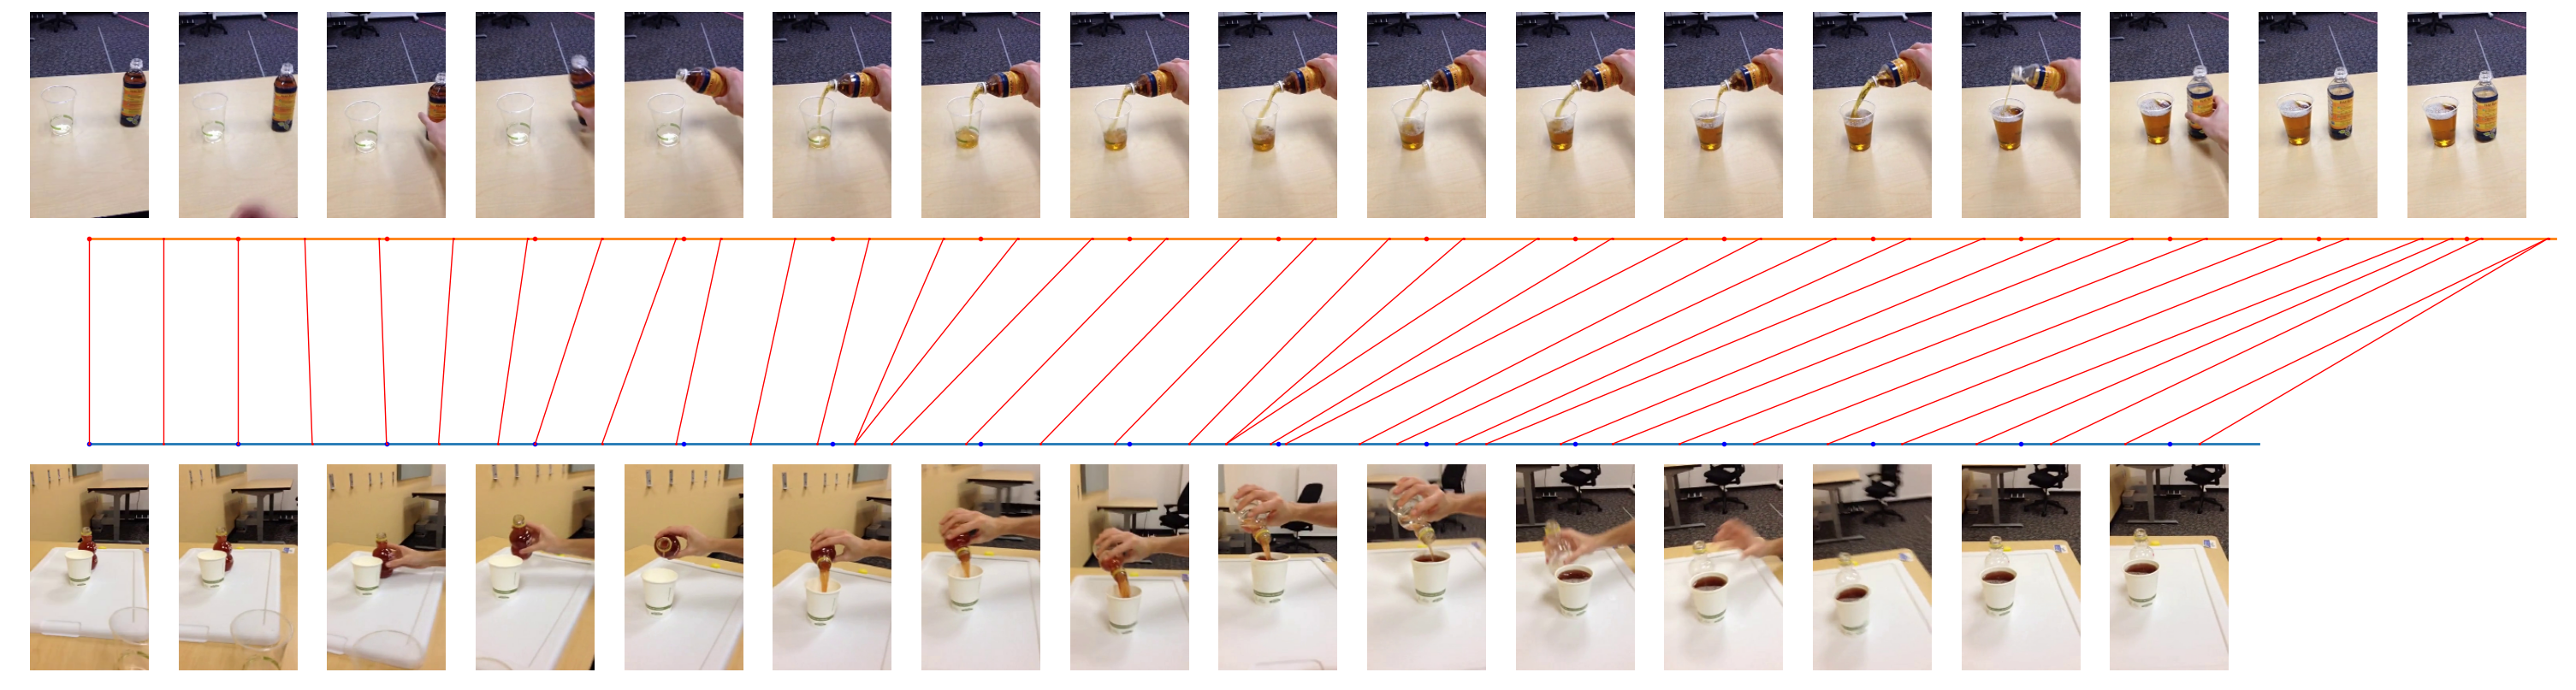
\includegraphics[width=0.764\textwidth]{images/v2.png}
% \\
% (a)&(b)
\end{tabular}
\caption{Similarity matrix (left) shows video alignment using an optimal path and the respective video aligned frame-by-frame (right).}
\label{fig: vis_align}
\end{figure}

\noindent \textbf{Results on PennAction Dataset.} 
Table \ref{tab: pn_class} compares the performance of our method with state-of-the-art approaches on the PennAction dataset. Bold and underlined text denote the best and second-best results. 
LAC consistently outperforms previous methods across most metrics, with the exception of Kendall's Tau. 
Notably, the improvement in AP@K is more pronounced on PennAction than on Pouring, likely due to the fewer number of frames in PennAction dataset, which may further impact alignment performance.

\begin{figure}[t]
\begin{tabular}{cc}
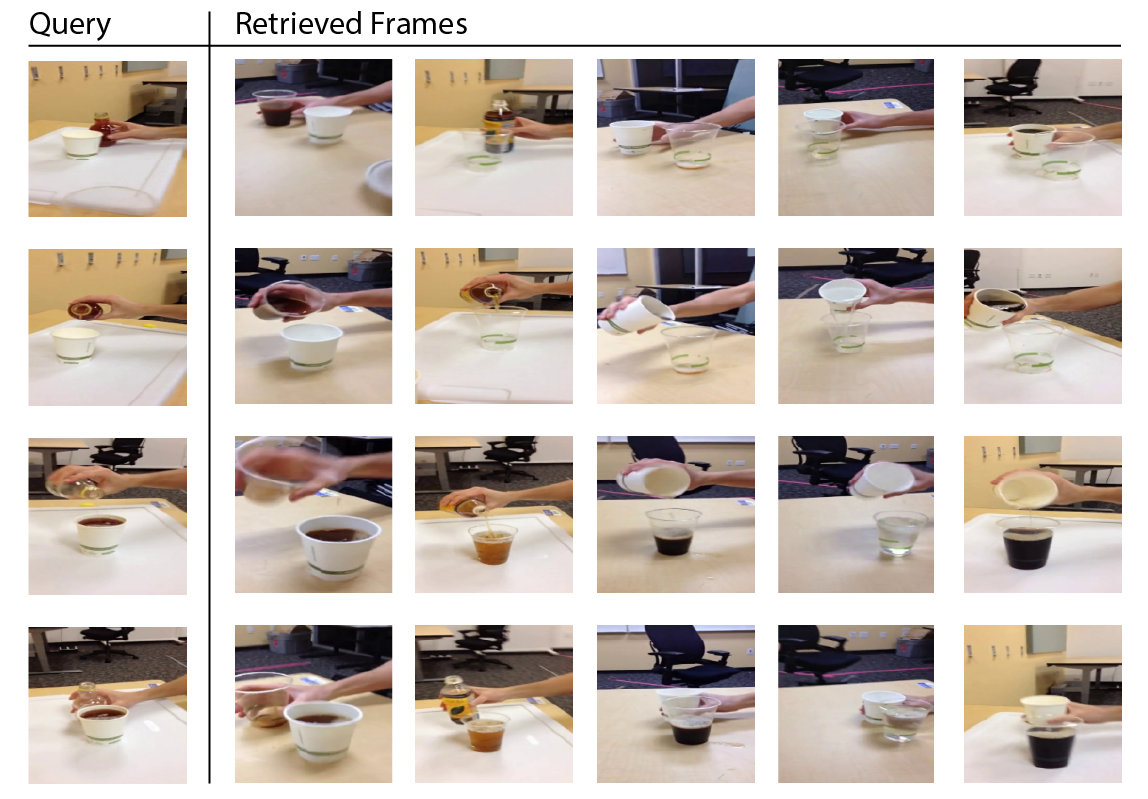
\includegraphics[width=0.45\textwidth]{images/v3.png}&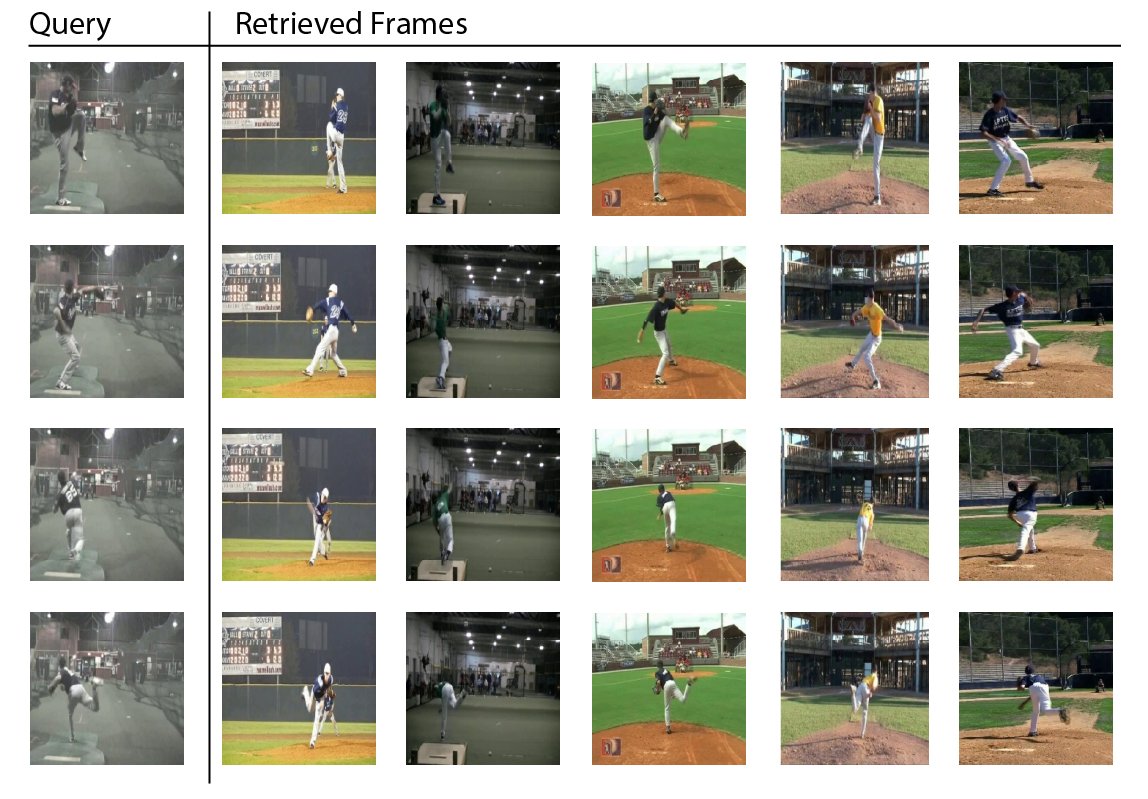
\includegraphics[width=0.45\textwidth]{images/v4.png}
% \\
% (a)&(b)
\end{tabular}
\caption{Fine-grained frame retrieval for Pouring (left) and PennAction (right) achieved using nearest neighbors within our embedding space.}
\label{fig: vis_retr}
\end{figure}

\noindent \textbf{Qualitative analysis of results.} 
Figure \ref{fig: vis_align} illustrates the alignment process, with the optimal path depicted on the left and the frame-by-frame alignment on the right. 
This visualization demonstrates the synchronization of the two videos despite differences in their temporal progression and duration. 
Such alignment visualizations enable in-depth analysis of deviations or inefficiencies within specific actions in video understanding.
Additionally, Figure \ref{fig: vis_retr} showcases our embedding-based retrieval system's ability to accurately identify and retrieve frames corresponding to specific action sequences across different videos.

\subsection{Ablation Study}

This section presents multiple experiments on the \textit{Pouring} dataset that analyze the different components of our framework. 

\begin{table}[H]
\small
\centering
\begin{tabularx}{0.99\linewidth}{|X|ccc|}
\hline
\textbf{Architecture} & \textbf{Class} & \textbf{Progress} & \textbf{$\tau$} \\
\hlineB{3}
ResNet-50 + Convolutional 3D & 88.04 & 73.26 & 71.37 \\
\hline
ResNet-50 + Tranformer 
(w/o pretrained weights) & 90.06 & 89.32 & 94.87 \\
\hline
ResNet-50 + Transformer
 & \textbf{95.16} & \textbf{94.24} & \textbf{97.50} \\
\hline
\end{tabularx}
\caption{Different Encoder Architecture on Model Performance.}
\label{tab_lac_arch}
\end{table}

\begin{table}[H]
\parbox{.4\linewidth}{
\centering
\begin{tabularx}{0.99\linewidth}{|c|ccc|}
\hline
\textbf{$\gamma$} & \textbf{Class} & \textbf{Progress} & \textbf{$\tau$} \\
\hlineB{3}
0.6 & 93.44 & 92.12 & 94.93 \\
\hline
0.7 & 94.87 & 92.82 & 97.29 \\
\hline
0.8 &  \textbf{95.16} & \textbf{94.24} & \textbf{97.50} \\
\hline
0.9 & 93.93 & 92.02 & 94.91 \\
\hline
\end{tabularx}
\caption{Different $\gamma$ Values on Model Performance}
\label{tab_lac_y}
}
\hfill
\parbox{.59\linewidth}{
\centering
\begin{tabularx}{0.99\linewidth}{|X|ccc|}
\hline
\textbf{Loss $\mathcal{L}$} & \textbf{Class} & \textbf{Progress} & \textbf{$\tau$} \\
\hlineB{3}
$\mathcal{L}_c $ & 93.44 & 92.12 & 94.93 \\
\hline
$\mathcal{L}_c + \alpha \cdot \mathcal{L}_l$ & 93.71 & 92.16 & 95.01 \\
\hline
$\mathcal{L}_c + \alpha \cdot (\mathcal{L}_l + \beta \cdot (\mathcal{L}_{sw12} + \mathcal{L}_{sw21}))$ & \textbf{95.16} & \textbf{94.24} & \textbf{97.50} \\
\hline
\end{tabularx}
\caption{Different LAC Loss Formulations on Model Performance}
\label{tab_lac_loss}
}
\end{table}

\noindent \textbf{Network Architecture.} Table \ref{tab_lac_arch} demonstrates that our performance evaluation across various network architectures highlights the superiority of the ResNet-50 model with pretrained weights combined with a Transformer.

\noindent \textbf{Hyperparameter of LAC Loss.} Table \ref{tab_lac_y} presents the optimal performance results obtained at the smoothing parameter $\gamma = 0.8$. 
Table~\ref{tab_lac_loss} further demonstrates that integrating local alignment loss into the total loss significantly enhances performance and achieves the highest scores across all metrics compared to using contrastive loss alone.
